\author{Tieyuan Zhu}
%%%%%%%%%%%%%%%%%%%%%
\title{Implementation aspects of attenuation compensation in reverse-time migration}

\righthead{Q-RTM}
\lefthead{Zhu}
%\footnote{Submitted to Geophysical Prospecting}

\begin{abstract}
Attenuation compensation in reverse time migration has been shown to improve the resolution of the seismic image. I study three essential aspects of implementing attenuation compensation in reverse time migration: the physical justification of attenuation compensation, the choice of imaging condition, and the choice of low-pass filter. The physical illustration of attenuation compensation supports the mathematical implementation by reversing the sign of the absorption operator and leaving the sign of the dispersion operator unchanged in the decoupled viscoacoustic wave equation. Further theoretical analysis shows that attenuation compensation in reverse time migration using the two imaging conditions (crosscorrelation and source-normalized crosscorrelation) is immune to attenuation effects. In numerical experiments using a simple-layered model, the crosscorrelation imaging condition may be preferable based on the criteria of amplitude corrections. The amplitude and phase recovery to some degree depend on the choice of a low-pass filter. In an application to a realistic Marmousi model with added Q, high-resolution seismic images with the correct amplitude and kinematic phase is obtained by compensating for both absorption and dispersion effects. Compensating for absorption only can amplify the image amplitude but with a shifted phase.
\end{abstract}

\section{Introduction}
To obtain high-resolution (even true-amplitude) seismic images, attenuation effects must be compensated for in seismic imaging. In conventional seismic data processing, inverse-Q filter is commonly used to mitigate attenuation effects in the data domain \citet[]{wang2002}. They are usually limited by simple 1-D $Q$ models. Wave equation based compensation is preferable because it is effective in balancing amplitudes for signals that have traversed paths of significantly different lengths as well as for paths that have experienced significantly different amount of amplitude loss due to heterogeneous attenuation in space.

In past decades, several efforts have been made to perform attenuation compensation in wave equation based seismic imaging. They apply wavefield extrapolation based on one-way wave equation \citep{Mittet1995, Zhang2002, Mittet2007} and reverse-time migration (RTM) imaging \citep{Fletcher2012}. Two-way wave equations for RTM include the damping viscoscalar wave equation \citep{Deng2007} and the standard linear solid model \citep{Deng2008}. Because attenuation effects include amplitude absorption and velocity dispersion, to compensate for them in seismic images requires taking care of both. However, the above formulations exhibit coupled attenuation operators. Therefore, these wave equations may not fully compensate for both absorption and dispersion effects. An alternative viscoacoustic wave equation based on pseudo-differential operators introduced by \citet[]{Zhang2010} might remedy this problem. 

\citet[]{zhu14a} derived a time-domain viscoacoustic two-way wave equation, which introduces explicitly decoupled absorption and dispersion operators. Using this wave equation, \citet[]{zhu14d} developed a Q-compensated RTM (Q-RTM) method to fully compensate for both absorption and dispersion. The Q-RTM method has been also applied to a crosswell field data for improving the image of the attenuative reservoir zone \cite[]{zhu15b}. The basis of Q-RTM method is that the decoupling property allows to treat absorption and dispersion differently when compensating for both effects by mathematically reversing the sign of amplitude loss term but leaving the sign of dispersion term unchanged in the viscoacoustic wave equation. 
In practice, the higher frequencies in recorded data (receiver wavefield) are invariably contaminated with noise. Attenuation compensation might amplify such unwanted frequency content. Therefore, it is important to carefully choose a filter to stabilize this compensating procedure. \citet[]{zhu14b} and \citet[]{zhu14d} employ a low-pass Tukey filter for the attenuation and dispersion operators. On the other hand, the correct imaging condition for RTM is quite important to obtain the physical and reliable amplitudes. Both source-normalized crosscorrelation \citep{zhu14b} and crosscorrelation imaging conditions \citep{zhu14d} are used in Q-RTM. The questions to what the optimal filter and the best imaging condition should be for $Q$-RTM remain open.

A motivation for this paper is to further discuss and elaborate some of the ideas presented previously in \citet[]{zhu14d}. First of all, I illustrate why decoupled attenuation operators are needed for compensating for amplitude absorption and dispersion in seismic imaging in a physical way. Compensating for only absorption or dispersion would not lead to the improvement of the image quality. I further compare two imaging conditions for $Q$-RTM based on the criteria of amplitude and kinematic phase and investigate how the filter choice affects this attenuation compensation. These implementation aspects of the $Q$-RTM method are essential for obtaining high-resolution seismic images. 

The paper is organized as follow. First, I demonstrate attenuation compensation by the inverse of absorption and the same dispersion in a physical way. Then, I review formulations of forward and backward propagation in a newly developed $Q$-RTM method by \citet[]{zhu14d}. In the second part, I analyze two imaging conditions from a theoretical point of view and show different implementations of two imaging conditions in $Q$-RTM. In numerical examples, I investigate the performance of two imaging conditions and a low-pass filter using a simple layered model. I then illustrate the importance of compensating for both amplitude loss and dispersion effects during RTM using the Marmousi model with added Q.


\section{Forward and backward propagation in attenuating media}

In this section, I first explain why we need to implement a different treatment to amplitude absorption and dispersion when compensating for attenuation effects during wave propagation. Then, I briefly review the viscoacoustic wave equation with decoupled attenuation operators. Finally, I explain the methodology for implementing back-propagation and compensating for attenuation effects using the adjoint constant-Q wave equation.

\subsection{Compensating for dispersion and absorption effects during backpropagation}

As shown schematically in the top of Figure 1, an explosive source (red star) sends a signal into an attenuating medium. The waveform experiences attenuation during the forward propagation. According to the principle of velocity dispersion in attenuating media, higher frequencies (labeled by $H$ in Figure 1) travel faster than lower frequencies (labeled by $L$in Figure 1). Therefore, at receivers high frequencies advance to lower frequencies in the recorded waveform data. To back propagate the recorded data, the recorded data are flipped in time. Now lower frequencies are in front of higher frequencies. Then, the reversed data is injected as the boundary condition at the receivers. If we can use the same velocity dispersion, i.e., higher frequencies will again travel faster than the lower frequencies, back-propagation will reconstruct the desired wavefields at each propagation time. All frequencies finally arrive simultaneously at the original source. If that is not the case, high frequencies never catch up with low frequencies. We cannot reconstruct the desired wavefields. 

At the same time, the amplitude needs to be increased to compensate for absorption. It means that we need to apply the ‘opposite’ amplitude absorption to boost the amplitude of the signal. During back-propagation with attenuation compensation, we apply the amplitude recovery rather than the amplitude absorption but the same dispersion effect. In the mathematical treatment, we reverse the sign of the absorption operator and leave the sign of the dispersion operator unchanged. Finally, the receiver wavefields can be reconstructed as the original one in the mirrored forward propagation time. For instance, the wavefield at forward propagation time t is equal to that at the backward propagation time  . 

Conventional viscoacoustic/elastic wave equations based on mechanical models, e.g., standard linear solid by \citet[]{carcione1988} and \citet[]{zhu13} or fractional derivatives \citep{carcione2002, carcione2010}, couple absorption and dispersion effects in one operator. It might not be possible to implement attenuation compensation with different signs for absorption and dispersion operators using conventional viscoacoustic/elastic wave equations.

 \begin{figure}[!htb]
   \centering
   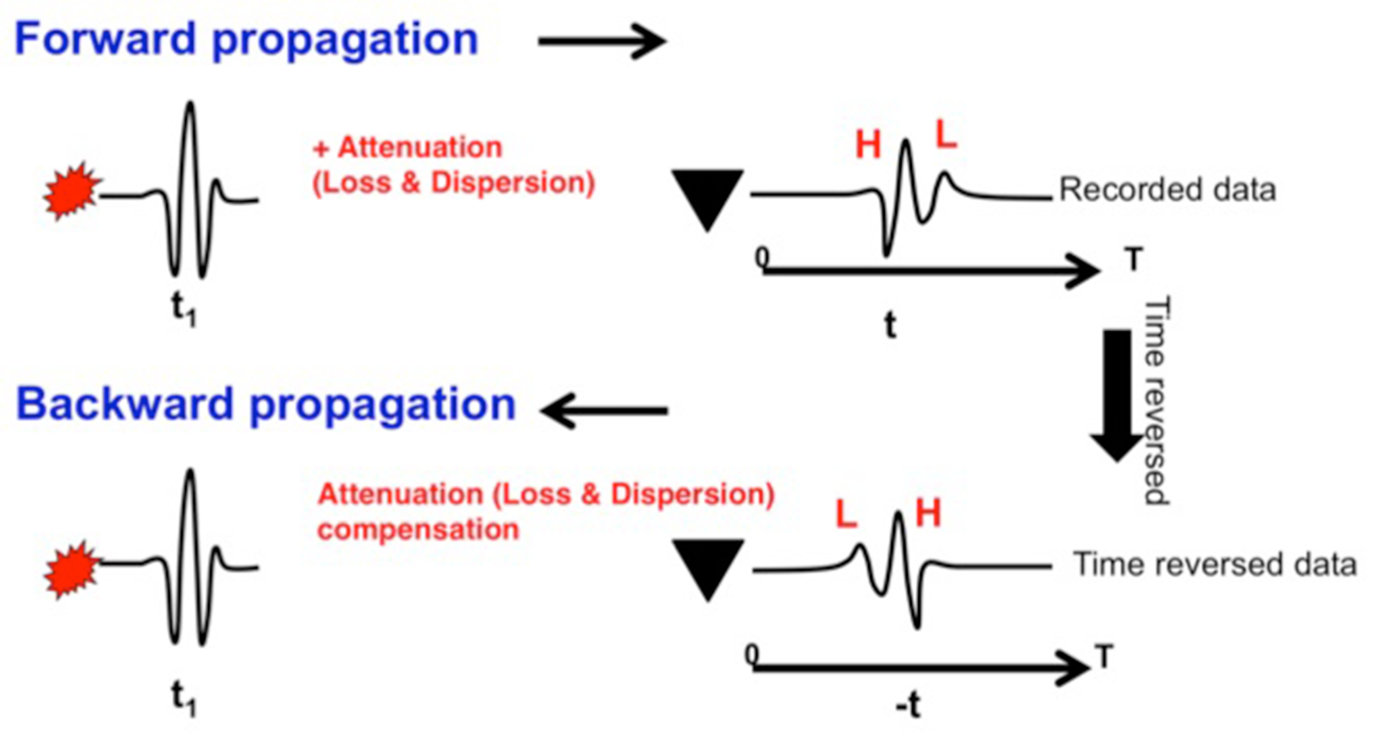
\includegraphics[width=0.8\textwidth]{Fig/fig1}
   \caption{Top: forward propagation in attenuating media; Bottom: backpropagation wavefield in attenuating media with attenuation compensation. The red star denotes an explosive source and the black triangulars denote receivers. The label \textbf{H} and \textbf{L} represent high frequencies and low frequencies signals. To correctly account for attenuation effects (including absorption and phase dispersion), the absorption term must be reversed so as to amplify the signal as time progresses. In contrast, the dispersion term (dependence of the sound speed on frequency) must remain unchanged.}
 \end{figure}

\subsection{Decoupled attenuation operators in viscoacoustic wave equation}

In order to compensate for such attenuation effects with treating amplitude loss and dispersion differently, I use a formulation of time-domain viscoacoustic wave equation based on the constant Q model \cite[]{kja79}, which was first introduced by \citet[]{zhu14a}. The most attractive feature of this formulation is the explicit separation of dispersion (second term in the right hand side) and absorption (third term). It is written as
\begin{equation}
  \label{eq:frac1}
 \frac{1}{c^2}\frac{\partial^2 p_{F}}{\partial t^2} = \nabla^2 p_{F} +  \left ( \eta \mathbf{L} - \nabla^2 \right ) p_{F}+ \tau \frac{\partial}{\partial t}\mathbf{H} p_{F}.
\end{equation}

The given source wavelet $S(t)$ is emitted at the source position ($x_s,z_s$),
\begin{equation}
\label{eq:eq2}                      
\hspace{0pt} P_{F}(x_s,z_s,t)=S(t),\hspace{\linewidth minus\linewidth}
\end{equation}

where $\mathbf{L}=\left ( -\Delta  \right )^{\gamma +1}, \mathbf{H}=\left ( -\Delta  \right )^{\gamma +1/2}$; $P_F$ is the spatial pressure field of forward modeling in time $t$ from 0 to T; and  $c_0$ is the acoustic velocity at the reference frequency $\omega_0$ . The operator coefficients are respectively given by

\begin{equation}
\label{eq:eq3}                      
\hspace{0pt} \eta = -c_0^{2\gamma}\omega_0^{-2\gamma}\cos(\pi \gamma) and \tau = -c_0^{2\gamma-1}\omega_0^{-2\gamma}\sin(\pi \gamma),\hspace{\linewidth minus\linewidth}
\end{equation}

where the variable $\gamma$ is defined as $\gamma=atan(Q^{-1})/\pi $. The range of $\gamma$ is $0<\gamma<0.5$ for any positive value of $Q$. The first term in the right side of equation (1) corresponds to the non-dispersive propagation operator. The second term corresponds to dispersion operator, and the third corresponds to absorption operator \cite[]{zhu14a}. In the following section, I show the advantage of this formulation in compensating for both dispersion and absorption effects in RTM. 

\subsection{Compensating for decoupled attenuation effects in RTM}

Mathematically, back propagation (time reversal) involves replacing time $t$ by $–t$ in equation (1). Accordingly, the viscoacoustic wave equation for back propagation is written as \cite[]{zhu14b}
\begin{equation}
  \label{eq4}
 \frac{1}{c^2}\frac{\partial^2 p_{B}}{\partial \hat{t}^2} = \nabla^2 p_{B} +  \left ( \eta \mathbf{L} - \nabla^2 \right ( p_{B}+ \tau \frac{\partial}{\partial \hat{t}}\mathbf{H} p_{B}.
\end{equation}

where  $\hat{t}=-t$ is the reversed time.  $p_B(x,-t)$ is a solution of equation (4) with the reversed sign of the absorption term. The positive sign of the absorption operator ($\beta=1$ ) represents the decay of amplitude in forward extrapolating source propagation as equation (1). Conversely, the sign of the first time derivative absorption term ($\beta=1$ ) is reversed, and thus it amplifies the amplitude. I emphasize that the second, dispersion-related term on the right hand side of equation (4) is time-independent and does not reverse the sign (i.e. the frequency-dependent phase velocity remains unchanged in time). This explanation also appears to justify why we treat dispersion and absorption operators differently. We will use equation (4) for extrapolating the source and receiver wavefields, correcting for attenuation and dispersion.

If we only consider the amplitude absorption effects and ignore phase dispersion effects, the absorption-dominated wave equation that contains the amplitude loss effects is written as
\begin{eqnarray}
  \label{eq5}
 \frac{1}{c^2}\frac{\partial^2 p_{B}}{\partial \hat{t}^2} = \nabla^2 p_{B} + \tau \frac{\partial}{\partial \hat{t}}\mathbf{H} p_{B}.
\end{eqnarray}
Similarly the dispersion-only wave equation can be obtained by dropping the third term in equation (4). Note that these two wave equations (absorption-only and dispersion-only) may not be physically correct and casual, but they are practically feasible for a numerical implementation. 
To prevent high-frequency noise from growing exponentially, I apply a low-pass filter to the dispersion and absorption operators in the spatial frequency domain when calculating the time-reversed wavefields. The numerical discretization of equations (4) and (5) is described in \citet[]{zhu14a}.

\section{IMAGING CONDITIONS}
In this section I consider the implementation of two imaging conditions – crosscorrelation and source-normalized crosscorrelation, for Q-compensated RTM (Q-RTM). I conduct a theoretical analysis based on plane waves. 
 \begin{figure}[!htb]
   \centering
   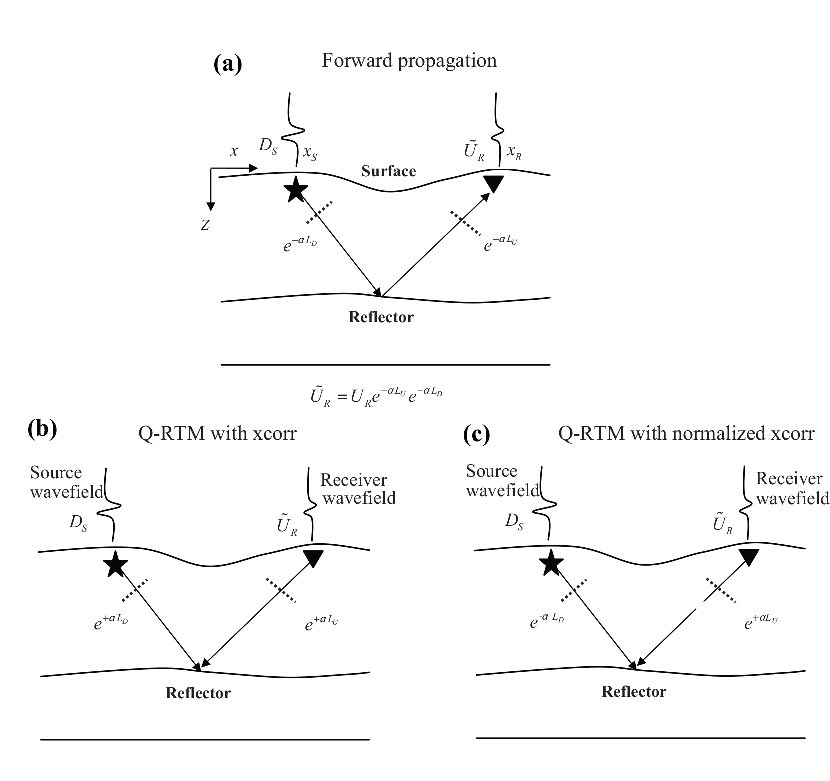
\includegraphics[width=0.8\textwidth]{Fig/fig2-eps-converted-to}
   \caption{Schematic illustration of forward propagation in attenuating media (a), Q-compensated RTM with crosscorrelation (b), and source-normalized crosscorrelation (c) imaging conditions.}
 \end{figure}

Figure 2a illustrate that seismic waves are attenuated in the subsurface. We assume that seismic waveform is attenuated by the exponential rate  $e^{-\alpha L}$, where $L$ is the propagation distance. The waves travel from the source to reflectors in $L_{D}$  and then reflect back to receivers in $L_{U}$ . The total attenuation along the accumulated wavepath is $e^{-\alpha L_D}e^{-\alpha L_U}$ , where the subscripts $D$ and $U$ denote the downgoing and upgoing waves, respectively. The receiver wavefield at any point   in the imaging space is calculated by  $\tilde{R}(\mathbf(x),t)=R(\mathbf(x),t)e^{-\alpha L_D}e^{-\alpha L_U}$.  $R(\mathbf(x),t)$ is the backward propagated receiver wavefields at time t in a non-attenuating medium.

Intuitively, to compensate for both phase dispersion and amplitude loss in the wavefield at the receivers, the measured receiver wavefield should be compensated by the gain factor  $e^{+\alpha L_D}e^{+\alpha L_U}$. Note that the dispersion effects are taken care of by propagating wavefields in the forward and backward using equation (4). 

\subsection{Crosscorrelation}
For the crosscorrelation-based RTM algorithm, \citet[]{zhu14d} propose to design compensation operators for both the source and receiver wavefields; that is, to apply compensation  $e^{+\alpha L_D}$ for extrapolating the source wavefield  from source to reflector and compensation  $ e^{+\alpha L_U}$ for extrapolating the receiver wavefield $S(\mathbf{x},t)$ from receiver to reflector, as illustrated in Figure 2b. Along the wavepath where the attenuation effects accumulate, the source wavefield  $S(\mathbf{x},t)$ is compensated to $S^{C}(\mathbf{x},t)$  after propagating the distance $L_D$  as shown in Figure 2b:
\begin{equation}
\label{eq:eq6}                      
\hspace{0pt} S_{C}(\mathbf{x},t)=S(\mathbf{x},t),\hspace{\linewidth minus\linewidth}
\end{equation}

where $S(\mathbf{x},t)$  represents the source wavefield in a non-attenuating medium. The receiver wavefield amplitude  $\tilde{S}(\mathbf{x},t)$ at grid point of the reflector is compensated to $R^{C}(\mathbf{x},t)$  at each time step using
\begin{equation}
\label{eq:eq7}                      
\hspace{0pt} R_{C}(\mathbf{x},t)=\tilde{R}(\mathbf{x},t)e^{+\alpha L_U},\hspace{\linewidth minus\linewidth}
\end{equation}
With equation (6) and equation (7), I apply the crosscorrelation imaging condition at each image point to obtain, 
\begin{eqnarray}
\label{eq:eq8}                      
I_{C}(\mathbf{x})=\int_{a}^{b} S_{C}(\mathbf{x},t)R_{C}(\mathbf{x},t) dt = \int_{a}^{b} S(\mathbf{x},t) \tilde{R}(\mathbf{x},t) e^{+\alpha L_D}e^{+\alpha L_U}dt \\
= \int_{a}^{b} S(\mathbf{x},t) R(\mathbf{x},t) dt,\nonumber
\end{eqnarray}

where the compensated image $I_{C}(\mathbf{x})$  from the zero-lag crosscorrelation imaging condition is theoretically equivalent to  $I(\mathbf{x})$  of the non-attenuated acoustic RTM ( $I(\mathbf{x})=\int_{a}^{b} S(\mathbf{x},t) R(\mathbf{x},t) dt$ ). In other words, the image $I_{C}(\mathbf{x})$   is theoretically immune to attenuation and dispersion effects. Note that the crosscorrelated Q-RTM image has no physical interpretation as a reflection coefficient. 

\section{Source-normalized crosscorrelation}

Alternatively, the source-normalized crosscorrelation imaging condition is considered to produce the physically correct reflection coefficient \citep{claerbout1971, chatt2008}:
\begin{equation}
\label{eq:eq9}                      
\hspace{0pt} I_{C}(\mathbf{x})=\frac{\int_{a}^{b} S_{C}(\mathbf{x},t) R_{C}(\mathbf{x},t) dt}{\int_{a}^{b} S_{C}(\mathbf{x},t) S_{C}(\mathbf{x},t) dt}, \hspace{\linewidth minus\linewidth}
\end{equation}

With this imaging condition, the source wavefield will be attenuated rather than compensated for (Deng and McMechan 2007). Thus, the source wavefield will be computed in attenuating media by using equation (1) as shown in Figure 2c:
\begin{equation}
\label{eq:eq10}                      
\hspace{0pt} S_{C}(\mathbf{x},t)=S(\mathbf{x},t) e^{-\alpha L_D},\hspace{\linewidth minus\linewidth}
\end{equation}
The compensated receiver wavefield is defined in equation (7). The compensated image by source-normalized crosscorrelation is written as

\begin{equation}
\label{eq:eq11}                      
I_{C}(\mathbf{x})=\frac{\int_{a}^{b} S(\mathbf{x},t) e^{-\alpha L_D} \tilde{R}(\mathbf{x},t) e^{+\alpha L_U} dt }{\int_{a}^{b} S(\mathbf{x},t)e^{-\alpha L_D} S(\mathbf{x},t) e^{-\alpha L_D} dt } = \frac{\int_{a}^{b} S(\mathbf{x},t)  R(\mathbf{x},t) dt }{\int_{a}^{b} S(\mathbf{x},t) S(\mathbf{x},t) dt },
\end{equation}
In theory, the resulting image $I_{C}(\mathbf{x})$ from the attenuated source wavefield and the compensated receiver wavefield will be quantitatively interpreted as the reflection coefficient and qualitatively equivalent to the final image by equation (8). 
Based on equations (8) and (11), we conclude that $Q$-RTM with both imaging conditions results in a corrected amplitude and phase image compared with the reference image by acoustic RTM without attenuation in the data.

\section{Synthetic examples}

In the first experiment, I will consider a simple two-layer model to demonstrate the performance of crosscorrelation and source-normalized crosscorrelation imaging conditions. The velocity model consists of two layers shown in Figure 3a. The quality factor is $Q=30$ and density is $2200 kg/m_3$. The size of the model is a $100\times 200$  grid, with a grid spacing of $\Delta x=\Delta z=10$ m. A 200 m PML boundary is included at the edges of the model to reduce edge reflections. I place $20$ sources at a depth of 50 m. The source is a Ricker wavelet with a center frequency of $25$ Hz and onset time  $ t_0=0.04 $s. The time step is $1$ ms. The shot interval is $100$ m, whereas the receiver spacing is 10 m, with a total of 198 receivers located at a depth of 50 m. A sample shot gather is shown in Figure 3b. I plot the power spectrum of the first shot gather data (red curve) and its cutoff frequency in Figure 3c. Figure 3d shows an example of a 1D frequency-domain Tukey filter for taper ratios of 0.4 and 0.2 and a cutoff frequency of $120$ Hz. For RTM input, the velocity model is first smoothed. The parameters needed for Q-RTM are the reference frequency $1500$ Hz, the cutoff frequency of the low-pass Tukey filter 120 Hz, and a taper ratio of $0.2$.

 \begin{figure}[!htb]
   \centering
   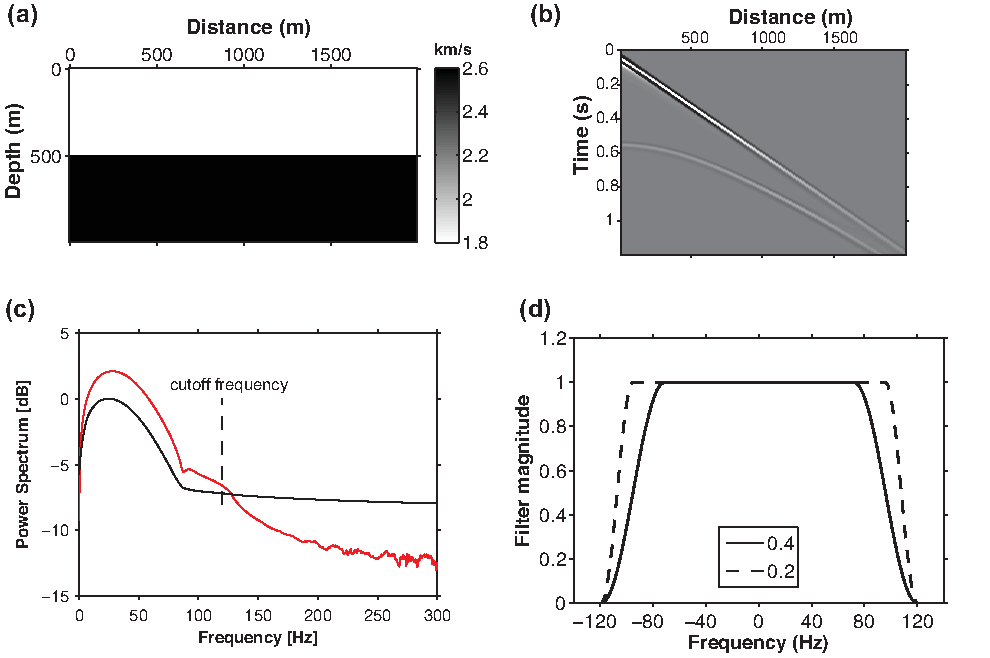
\includegraphics[width=0.8\textwidth]{Fig/fig3-eps-converted-to}
   \caption{(a) Velocity model; (b) common shot gather in the first shot position; (c) the power spectrum of single common shot data in (b), the dashed line denotes the cutoff frequency of 120 Hz. The solid black curve denotes the power spectrum of all common shot data; (d) 1D symmetric Tukey window with a frequency cutoff of 120 Hz and taper ratios of 0.4 (solid line) and 0.2 (dashed line).}
 \end{figure}

Figure 4 shows migrated images using crosscorrelation (left) and source-normalized crosscorrelation (right) imaging conditions. The first row (Figures 4a and 4d) shows the reference images by acoustic RTM of acoustic data. The second row (Figures 4b and 4e) shows the images by acoustic RTM of viscoacoustic data. With attenuation compensation, the reflectors by both imaging conditions are better imaged closer to the reference (Figures 4c and 4f). Using source-normalized imaging condition, the imaged reflector is visually thinner and thus higher resolution than that in the crosscorrelated image. Both images suffer from some artifacts around sources near the surface.

 \begin{figure}[!htb]
   \centering
   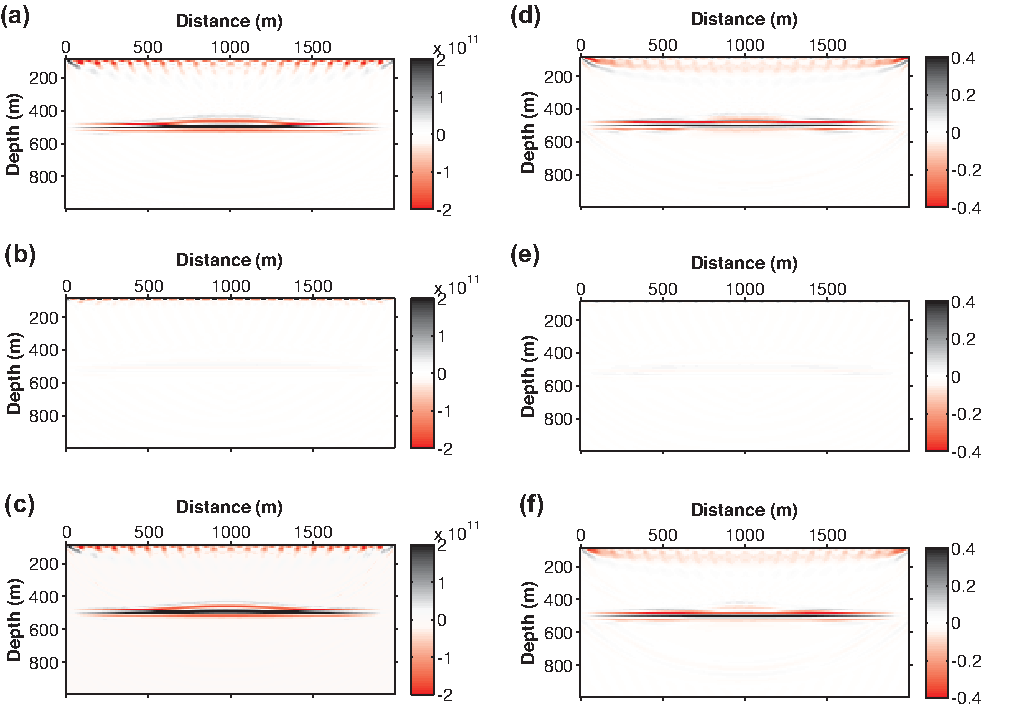
\includegraphics[width=0.8\textwidth]{Fig/fig4-eps-converted-to}
   \caption{Migrated images using crosscorrelation (left column) and source-normalized crosscorrelation (right column) imaging conditions. (a, d) reference images; (b, e) RTM images; (c, f) Q-RTM images. }
 \end{figure}

 \begin{figure}[!htb]
   \centering
   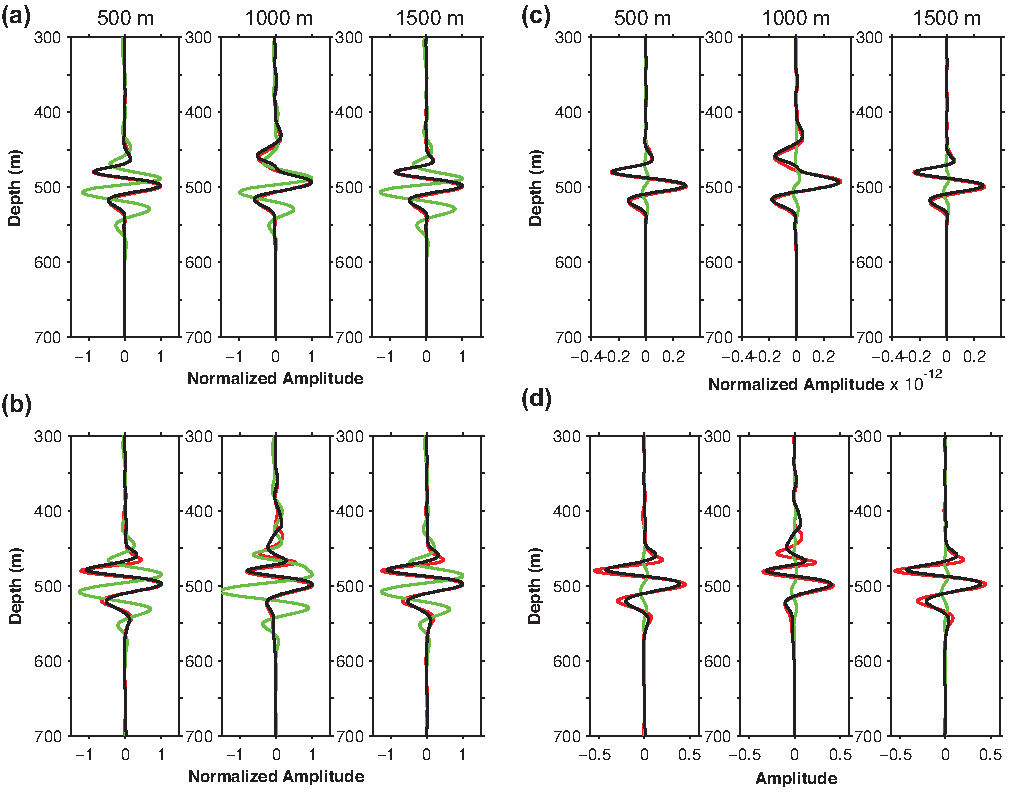
\includegraphics[width=0.8\textwidth]{Fig/fig5-eps-converted-to}
   \caption{Phase (a,b) and amplitude (c,d) of the reflector in Figure 4 by using crosscorrelation (a,c) and source-normalized crosscorrelation (b,d) imaging condition. }
 \end{figure}

To evaluate the results quantitatively, I show cross-sections of these images in Figure 5. Figures 5a and 5b compare the kinematic phase of the reflector at 500 m, 1000 m, and 1500 m by normalizing the traces by their maximum values while Figures 5c and 5d compare the amplitude information. Clearly, the amplitude and phase of the reflector by Q-RTM (black) with both crosscorrelation and source-normalized crosscorrelation are closer to the references (red). Without attenuation compensation, the imaged reflector is shifted from the true location of the reflector. Using the source-normalized crosscorrelation imaging condition the compensated amplitude (black) shows some errors to the reference amplitudes (red) in Figure 5d.
Further, Figure 6 shows the peak amplitude along the reflector in the horizontal direction. The amplitude from the crosscorrelated image in Figure 6a shows the recovered amplitude of the reflector. Using source-normalized crosscorrelation imaging condition, the main effect seems to be a slightly better recovery of constant amplitudes along the top reflector (Figure 6b), but there is a pronounced difference. These tests conclude that both imaging conditions for $Q$-RTM have the similar performance in phase but the crosscorrelated image gives better amplitude recovery compared to the reference image. 

 \begin{figure}[!htb]
   \centering
   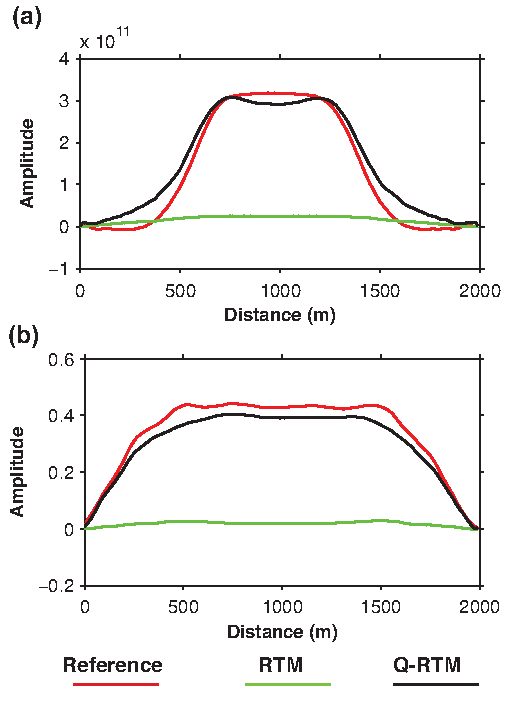
\includegraphics[width=0.8\textwidth]{Fig/fig6-eps-converted-to}
   \caption{Peak amplitude information of the reflector in Figure 4 by using crosscorrelation (a) and source-normalized crosscorrelation (b) imaging condition. }
 \end{figure}

In the following tests, I vary the cutoff frequency and taper ratio of low-pass Tukey filter to investigate how these filter parameters influence the amplitude and phase recovery. I use the crosscorrelation imaging condition. The cutoff frequency of the low-pass filter is determined by identifying a value based on the noise level of spectrum of the observed data (see Figure 3c). I select three different cutoff frequencies: (a) 60 Hz, (b) 90 Hz, and (c) 120 Hz. Figure 7a shows the recovered amplitude of the reflector. It is not surprising that the higher cutoff frequency results in the better amplitude recovery. Figure 7b shows the phase by using three different cutoff frequencies. Higher cutoff frequency tends to give better phase, though they all appear very close. It is important to note that, even with a low cutoff frequency (even lower than 60 Hz, though they are not shown here), the amplitude and phase are still better improved than that without compensation (green line in Figure 5 and 6a). Figure 8 shows the recovered amplitude (a) and phase (b) of the reflector with three different taper ratio values: (a) 0.6, (b) 0.4, and (c) 0.2. The taper ratio 0.2 of the Tukey filter gives the best results based on the amplitude and phase. This choice can be explained by Figure 3d. 

 \begin{figure}[!htb]
   \centering
   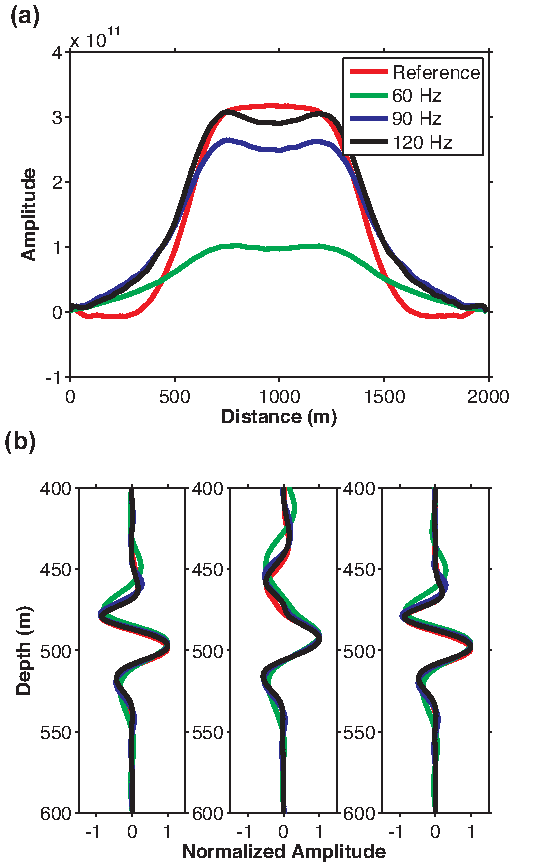
\includegraphics[width=0.8\textwidth]{Fig/fig7-eps-converted-to}
   \caption{Peak amplitude (a) and phase (b) of the reflector varying with the cutoff frequency of low-pass Tukey filter: 60 Hz (green), 90 Hz (blue), 120 Hz (black). The taper is 0.2 for all runs.}
 \end{figure}

 \begin{figure}[!htb]
   \centering
   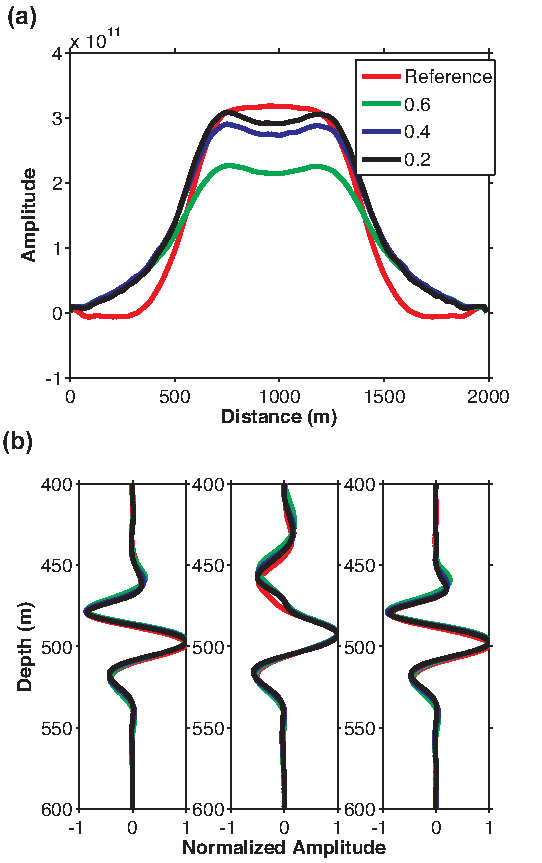
\includegraphics[width=0.8\textwidth]{Fig/fig8-eps-converted-to}
   \caption{Peak amplitude (a) and phase (b) of the reflector varying with the taper ratio of low-pass Tukey filter: 0.6 (green), 0.4 (blue), and 0.2 (black). The cutoff frequency of low-pass Tukey filter is 120 Hz for all runs.}
 \end{figure}

\subsection{Marmousi attenuation model} 
In this section, I test if compensating for both absorption and dispersion can improve the image resolution in amplitude and kinematic phase. For comparison, I also run absorption-only compensation. 


Figure 9 shows the Marmousi velocity model and added $Q_p$ models. The top high attenuation zones are typically caused in practice by the presence of gas chimneys. The size of the model is a $281\times 1001$ grid, with a grid spacing of  $\Delta x=\Delta z=12.5$ m. A 20-grid PML absorbing boundary on the four sides eliminates edge reflections. There are 97 sources, with each source being a Ricker wavelet with a center frequency of 20 Hz. The time step is 1 ms. The shot interval is 125 m, whereas the receiver spacing is 12.5 m with a total of 959 receivers. Sources and receivers are located at a depth of 62.5 m. Two synthetic datasets - acoustic ($Q\rightarrow infinite$) and viscoacoustic – were calculated using a forward modeling scheme using equation (1). I performed both acoustic RTM and the proposed Q-RTM. I chose a Tukey filter with a cutoff frequency of 120 Hz and a taper ratio of 0.1 to suppress the noise growth when running attenuation compensation. 
For comparison, I generated the reference image in Figure 10a by migrating acoustic data using acoustic RTM. I used acoustic RTM to migrate viscoacoustic data as a noncompensated case in Figure 10b. Without attenuation compensation the amplitude overall is weaker, especially the structure beneath the gas chimney zone (below depth 1.5 km). The anticline structures around the depth of 2 km disappear. The zoomed images in Figure 11 corresponding to Figure 10 show more details. Note that the noncompensated image in Figure 11b was scaled by the factor of 10. Although the overall amplitude of the image seems to be boosted, the anticline structures appear discontinuously and the top structures are distorted. To compare the phase of these images, I normalized traces at 7 km of the reference (red) and noncompensated images (green). The green line appears shifted from the reference red line. These features are clearly caused by uncompensated attenuation in the data. 

 \begin{figure}[!htb]
   \centering
   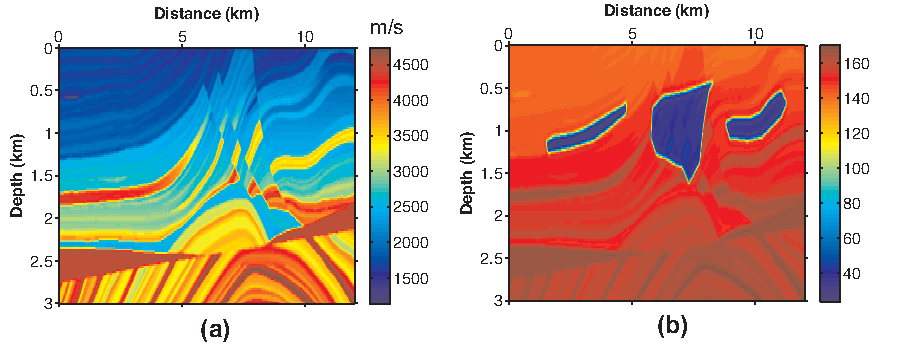
\includegraphics[width=0.8\textwidth]{Fig/fig9-eps-converted-to}
   \caption{P-wave velocity (a) and Q (b) Marmousi models. In the right panel (b), the blue zones indicate low-Q (high attenuation) gas cloudy areas.}
 \end{figure}

 \begin{figure}[!htb]
   \centering
   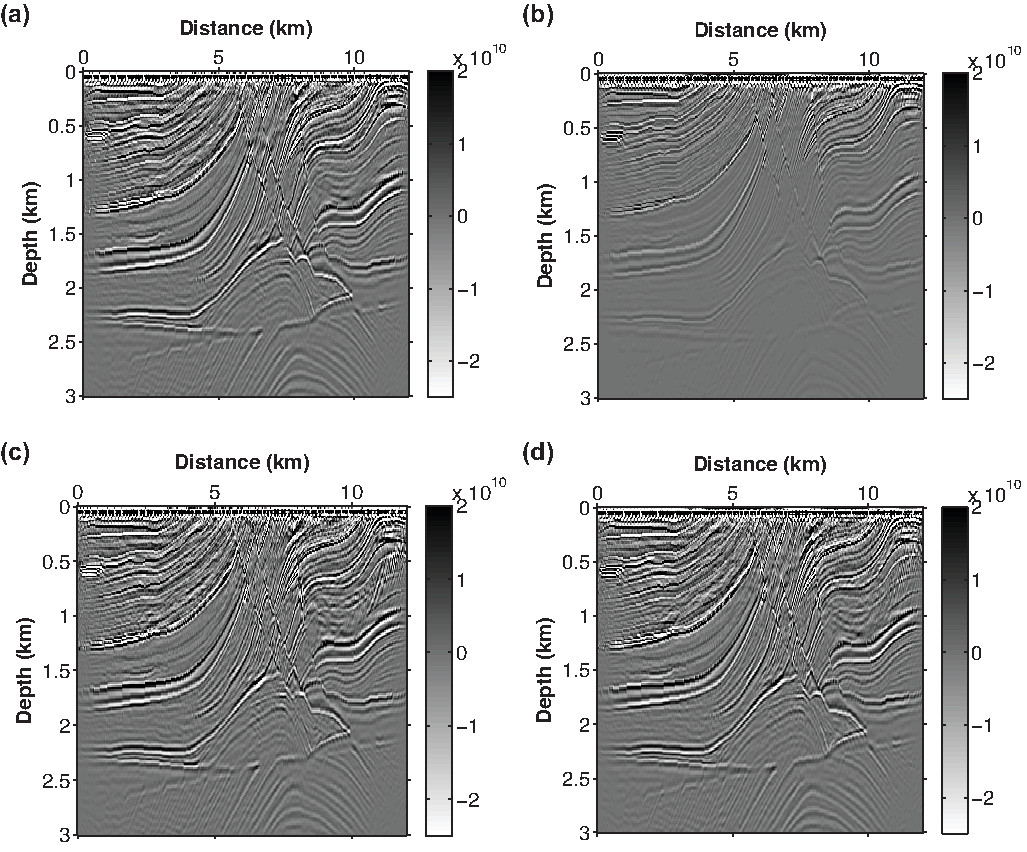
\includegraphics[width=0.8\textwidth]{Fig/fig10-eps-converted-to}
   \caption{(a) Acoustic RTM of acoustic data. (b) Acoustic RTM of viscoacoustic data. (c) Absorption-only compensated RTM with viscoacoustic data. (d) Q-compensated RTM with viscoacoustic data. All compensations are regularized by a low-pass Tukey filter with a cutoff frequency of 120 Hz. I used the crosscorrelation imaging condition.}
 \end{figure}

\subsubsection{Compensating for absorption only}
To show why the dispersion effect is important in the image, I deliberately used the nondispersive operator   rather than the dispersive operator (equation 5), thus, the velocity is nondispersive in the computational frequency range. I reversed the sign of the absorption operator and reran Q-RTM as above. The image result is shown in Figure 10c and its zoomed image is shown in Figure 11c. Clearly, the amplitude after absorption-only compensation only is boosted and the imaged anticline structure is continuous and can be tracked. Note that I use equation (5) to simulate both the forward propagated wavefield and backward propagated wavefield. If the forward modeling would use equation (1) instead of the absorption wave equation (5), the amplitude of the image would not be enhanced because of phase shifts between source and receiver wavefields (Zhu 2014b). To compare the phase of these images, I plot cross-sections at the lateral distance of 7 km in Figure 11e. Clearly, the green lines show the details of how the absorption-only-compensated image is off from the ground truth. 

 \begin{figure}[!htb]
   \centering
   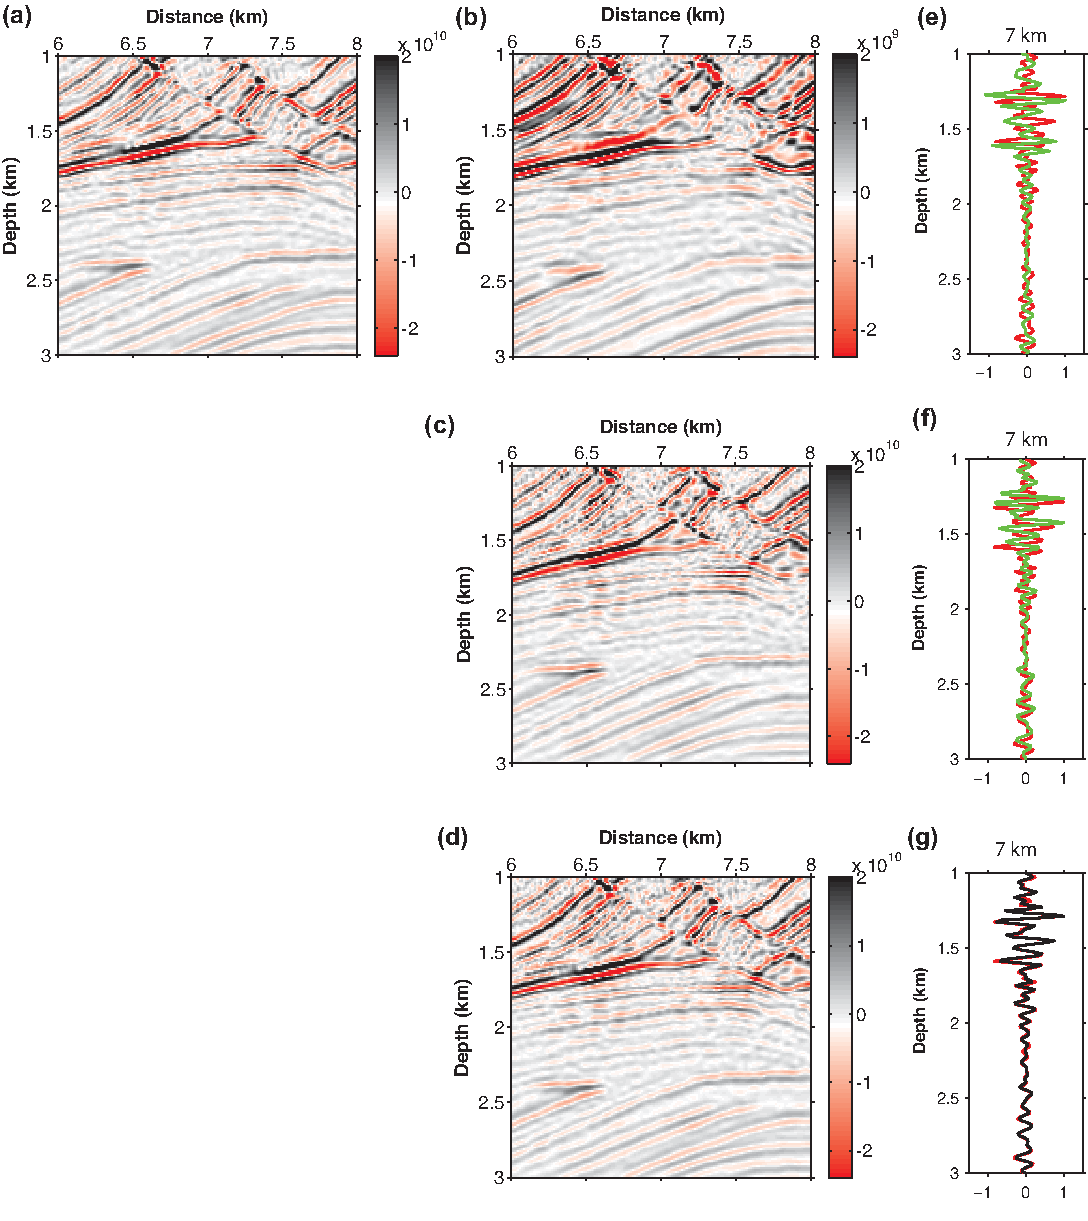
\includegraphics[width=0.8\textwidth]{Fig/fig11-eps-converted-to}
   \caption{Zoomed seismic images corresponding to Figure 10. Note that the image in Figure 11b is amplified by factor of 10. With compensating for both dispersion and absorption in Figure 11d, the imaged anticline structure below depth 1.5 km is continuously tracked while these are discontinuous in Figure 11b. Also the top part is better imaged in Figure 11d. The left panels show their corresponding normalized traces at the lateral distance of 7 km to compare the phase. With full compensation, the black line in Figure 11g gives best match to the reference red line.}
 \end{figure}

\subsubsection{Compensating for both absorption and dispersion}
By compensating for both absorption and dispersion, I plot the Q-compensated image in Figure 10d and its zoomed image in Figure 11d. The compensated image overall shows a recovered amplitude, especially in the deep areas. The top of anticline below the gas chimney zone appears to be better illuminated. The image resolution of the complex thin layer inside the gas chimney zone is significantly improved with better interface continuity. Compensation is effective in amplitude balancing for the whole image. The phase after attenuation compensation (black line) in Figure 11g matches that of the reference image (red line) remarkably well. 

To make quantitative comparisons of amplitudes for these images, I plot the true amplitudes of these images at the lateral distances of 6 km, 7 km, and 8 km in Figure 12. The top subfigure in Figure 12 is comparing traces of the RTM image (green) and Q-RTM image (black). The amplitude in the green line (no compensation) is very small compared to others. It is hard to identify the structure variations at the shown scale. The bottom subfigure is comparing traces of the absorption-compensated RTM (green) and Q-RTM image (black). It is not surprising that the absorption-compensated RTM (green) gives the amplified amplitude comparable to the reference image (red), although it has shifts in phase. The full attenuation compensation results in a greatly improved matching of traces to the reference ones in amplitude and phase.
%%========
\sideplot{fig12-eps-converted-to}{width=0.9\textwidth}{Comparison of true amplitude at the lateral distances of 6 km, 7 km, and 8 km in images in Figure 11. The red lines represent the reference traces. The black lines correspond to the fully compensated traces. In the top subfigures the green lines denote no compensation and the bottom green lines denote only absorption compensation. The reference image trace is in the red line and the compensated image traces are in black. }


To fully compare the two imaging conditions, I further applied RTM and Q-RTM based on the source-normalized crosscorrelation imaging condition. Figure 13c shows the Q-compensated image and Figure 14c shows the corresponding zoomed image. Compared with RTM images, Q-RTM exhibits similar benefits on the recovery of the amplitude and phase of imaged structures (Figure 13), especially the anticline structure beneath the gas chimney zone. Compared to the images by crosscorrelation in Figure 10 and Figure 11, the images by source-normalized crosscorrelation effectively balance overall amplitudes of deep reflectors but contain some high-frequency ringing artifacts. Zoomed images in Figure 14 verify the above observations. Traces at the lateral distance of 6 km, 7 km, 8 km are shown in Figure 15. In the top panel, the traces imaged by Q-RTM contain errors in amplitude, which is consistent with the observation in the first example. In the bottom panel, the kinematic phase of the Q-RTM image is recovered well (black line) comparing with the reference phase (red line).


%%===========
\plot{fig13-eps-converted-to}{width=0.9\textwidth}{Focused image of the horizontal force source by (a) elastic TR imaging with elastic seismograms; (b) elastic TR imaging with viscoelastic seismograms; (c) viscoelastic TR imaging with viscoelastic seismograms. Observe that elastic imaging does not even recover the correct sign of the amplitude. Horizontal (d) and vertical (e) cross-sections of focused images through the origin are compared. }


\plot{fig14-eps-converted-to}{width=0.9\textwidth}{P-wave velocity (a) and Qp (b) models with the receiver array in the right-hand well, with the source area indicated by the white dashed line area.}


%%=======
\plot{fig15-eps-converted-to}{width=0.6\textwidth}{Source images by elastic and viscoelastic TR imaging. These images are produced by (a) elastic TR imaging with the elastic data; (b) elastic TR imaging with the viscoelastic data; (c) viscoelastic TR imaging with the viscoelastic data. The corresponding zoomed images of the source area are shown in (d), (e), and (f). The white dashed line area indicates the desired source area. These images are displayed in the same color scale. }


\section{Conclusion}
Q-compensated reverse-time migration is a promising method for improving the image resolution in amplitude and phase. The core step of this migration method is to fully compensate for attenuation effects (absorption and dispersion). Such compensation is done by reversing the sign of absorption operator and leaving the sign of the phase dispersion operator unchanged in the viscoacoustic wave equation with decoupled attenuation operators. It is worth noting that the commonly ignored phase dispersion as well as the absorption effect contribute to the recovery of both the kinematic phase and the amplitude of seismic images. Compensating for absorption only can recover the image amplitude but produces a wrong phase. 
With the crosscorrelation imaging condition, attenuation compensation should be applied to both forward and backward modeling. With the source-normalized crosscorrelation imaging condition, attenuation compensation is only applied in backward modeling while attenuation is applied in forward modeling. From numerical examples, we conclude that both imaging conditions show similar performance in the kinematic phase. The amplitudes in the crosscorrelated image better match the amplitude of the reference image, though these amplitudes are not physically meaningful. 
The amplitude and phase recovery to some degree depend on the choice of a low-pass filter. A higher cutoff frequency can bring higher frequencies into the compensation processing. At the same time, it can amplify the high-frequency noise. It is crucial for real data to select a suitable cutoff frequency for imaging, because of the low signal-to-noise ratio, which may lead to a lower cutoff frequency based on the noise level of the data spectrum. Even with a lower cutoff frequency, however, the proposed method of attenuation compensation during migration still improves the resulting images compared to the images without compensation.

\section{Acknowledgements}
I would like to thank Sergey Fomel, editors, and two reviewers for critical comments on the manuscript. The author is financially supported by Jackson Distinguished Postdoctoral Fellowship at the University of Texas at Austin. 

\newpage
\bibliographystyle{seg}
\bibliography{ref032015}

